\begin{frame}
	\frametitle{Números binários}
	\begin{columns}
		\column{0.6\textwidth}
			\par Vantagens
			\begin{itemize}
				\item Dois estados (mais difícil deteriorar)
				\item Discretos
				\item Manipulação algébrica (álgebra de Boole)
			\end{itemize}
		\column{0.4\textwidth}
			\par Desantagens
			\begin{itemize}
				\item Dois estados em oposição a infinitos estados
				\item Discretos em oposição a contínuo
			\end{itemize}
	\end{columns}
	\par Mundo ideal: Junção do analógico com o digital
\end{frame}


\begin{frame}
	\frametitle{Sistema numérico posicional}
	
	\begin{columns}
		\column{0.5\textwidth}
			\par Dada a base com uma certa quantidade de elementos $B$ e símbolos $d \in D = \{d_0, \dots, d_n \}$, então um valor numérico decimal $V$ \textbf{posicional} pode ser representado por 
			\begin{equation}
				V(B) = \sum_{i=0}^{n} d_i . B^{n - i}
			\end{equation}
			\par Sendo $||$ o operador de cardinalidade então $n=|D| - 1$ \newline
		\column{0.5\textwidth}
			\only<1>{
				\par Por exemplo, para o número \textbf{decimal} 249:
				\par $B=10$ 
				\par $D = \{2,4,9\} \implies |D| = 3 \implies n = 2$
				\begin{equation}
					\begin{aligned}
						&V(10) = \sum_{i=0}^{2} d_i . 10^{2-i} = \\
						&d_0 . 10^{2-0} + d_1 . 10^{2-1} + d_2 . 10^{2-2} = \\
						&2 . 10^2 + 4 . 10^1 + 9 . 10^0 = \\
						&\boxed{2.100 + 4.10 + 9.1 = 249}
					\end{aligned}
				\end{equation}
			}
			\only<2>{
				\par Por exemplo, para o número \textbf{binário} 11:
				\par $B=2$ 
				\par $D = \{1,1\} \implies |D| = 2 \implies n = 1$
				\begin{equation}
					\begin{aligned}
						&V(2) = \sum_{i=0}^{1} d_i . 2^{1-i} = \\
						&d_0.2^{1-0} + d_1.2^{1-1} = \\
						&1.2^1 + 1.2^0 = \\
						&\boxed{2+1 = 3}
					\end{aligned}
				\end{equation}
			}
	\end{columns}
\end{frame}

\begin{frame}
	\frametitle{Circuitos lógicos e algébra Booleana}
	\par Antes de avançarmos no estudo e na representação de circuitos lógicos, vamos entender como os estados de "ligado" e "desligado" dos componentes podem ser utilizados para gerar resultados úteis. Portanto, antes de abordarmos esses tópicos, faremos uma imersão na álgebra booleana, explorando tabelas verdade e formas de composição.
\end{frame}

\begin{frame}
	\frametitle{Álgebra de Boole: Operadores \textbf{AND}, \textbf{OR} e \textbf{NOT}}
	\par Sendo o sistema binário posicional aplica-se a ele muitas das regras as quais podemos aplicar aos números decimais o que nos leva a Álgebra de Boole e seus operadores:\newline
	
	\only<1>{
		\begin{columns}
			\column{0.6\textwidth}
				\par \textbf{AND} denotado como \textbf{.} ou $\land$\newline
				\par O operador \textbf{AND} é uma função de 2 variáveis definida como:
				\begin{equation}
					\begin{aligned}
						&AND(a,b) = a.b \\
						&AND(a,b) = 1, \forall a=b=1 \\
						&AND(a,b) = 0, \forall a \neq b \\
					\end{aligned}
				\end{equation}
			\column{0.4\textwidth}
				\begin{table}[h!]
					\centering
					\begin{tabular}{|c|c|c|c|}
						\hline
						a & b & a . b \\ \hline
						0 & 0 & 0     \\ \hline
						0 & 1 & 0     \\ \hline
						1 & 0 & 0     \\ \hline
						1 & 1 & 1     \\ \hline
					\end{tabular}
				    \caption{Tabela verdade para \textbf{AND}.}
					\label{tab:tabelaVerdadeAND}
				\end{table}
		\end{columns}
	}
	\only<2>{
		\begin{columns}
			\column{0.6\textwidth}
				\par \textbf{OR} denotado com \textbf{+} ou $\lor$\newline
				\par O operador \textbf{OR} é uma função de 2 variáveis definida como:
				\begin{equation}
					\begin{aligned}
						&OR(a,b) = a + b \\
						&OR(a,b) = 0, \forall a=b=0 \\
						&OR(a,b) = 1, \forall a \neq b, a=b=1 \\
					\end{aligned}
				\end{equation}
			\column{0.4\textwidth}
			\begin{table}[h!]
				\centering
				\begin{tabular}{|c|c|c|c|}
					\hline
					a & b & a + b \\ \hline
					0 & 0 & 0     \\ \hline
					0 & 1 & 1     \\ \hline
					1 & 0 & 1     \\ \hline
					1 & 1 & 1     \\ \hline
				\end{tabular}
    			\caption{Tabela verdade para \textbf{OR}.}
				\label{tab:tabelaVerdadeOR}
			\end{table}
		\end{columns}
	}
	
	\only<3>{
		\begin{columns}
			\column{0.6\textwidth}
			\par \textbf{NOT} denotado com $\overline{a}$ ou $\neg a$\newline
			\par O operador \textbf{NOT} é uma função de 1 variável definida como:
			\begin{equation}
				\begin{aligned}
					&NOT(a) = \overline{a} \\
					&NOT(a) = 0, \forall a=1 \\
					&NOT(a) = 1, \forall a=0 \\
				\end{aligned}
			\end{equation}
			\column{0.4\textwidth}
			\begin{table}[h!]
				\centering
				\begin{tabular}{|c|c|}
					\hline
					a & $\overline{a}$ \\ \hline
					0 & 1  \\ \hline
					1 & 0 \\ \hline
				\end{tabular}
				\caption{Tabela verdade para \textbf{NOT}.}
				\label{tab:tabelaVerdadeNOT}
			\end{table}
		\end{columns}
	}
\end{frame}

\begin{frame}
	\frametitle{Álgebra de Boole: Composição de de operadores}
	\par É importante destacar que assim com na álgebra tradicional os operadores tem prioridade no momento de sua aplicação na seguinte ordem: \textbf{NOT}, \textbf{AND} e por fim \textbf{OR}. Se usarmos os sinais as regras ficam bem parecidas com a álgebra tradicional: $\overline{a}$, $.$ e $+$.\newline
	
	\begin{columns}
		\column{0.4\textwidth}
			\par A partir dos operadores apresentados vamos brincar um pouquinho com eles:
			\begin{equation}
				(a + b) . c
			\end{equation}
		\column{0.6\textwidth}
			\begin{table}[h!]
				\centering
				\begin{tabular}{|c|c|c|c|c|}
					\hline
					a & b & c & a+b & \(a + b\) . c\\ \hline
					0 & 0 & 0 & 0 & 0 \\ \hline
					0 & 0 & 1 & 0 & 0 \\ \hline
					0 & 1 & 0 & 1 & 0 \\ \hline
					0 & 1 & 1 & 1 & 1 \\ \hline
					1 & 0 & 0 & 1 & 0 \\ \hline
					1 & 0 & 1 & 1 & 1 \\ \hline
					1 & 1 & 0 & 1 & 0 \\ \hline
					1 & 1 & 1 & 1 & 1 \\ \hline
				\end{tabular}
				\caption{Tabela verdade para \textbf{(a + b) . c}.}
				\label{tab:tabelaVerdadeComposta01}
			\end{table}
	\end{columns}
\end{frame}

\begin{frame}
	\frametitle{Álgebra de Boole: Composição de operadores NAND e NOR}
	\begin{center}
		Alguns operadores comuns são compostos: 
	\end{center}
	\begin{columns}
		\column{0.5\textwidth}
		
			\par O operador \textbf{NAND} (NOT AND) é definido segundo a seguinte tabela verdade:
		
			\begin{table}[h!]
				\centering
				\begin{tabular}{|c|c|c|c|c|}
					\hline
					a & b & a . b & $\overline{a . b}$ \\ \hline
					0 & 0 & 0     & 1  \\ \hline
					0 & 1 & 0     & 1  \\ \hline
					1 & 0 & 0     & 1  \\ \hline
					1 & 1 & 1     & 0  \\ \hline
				\end{tabular}
				\caption{Tabela verdade para \textbf{NAND}.}
				\label{tab:tabelaVerdadeNAND}
			\end{table}
		
		\column{0.5\textwidth}
			\par O operador \textbf{NOR} (NOT OR) é definido segundo a seguinte tabela verdade:
			\begin{table}[h!]
				\centering
				\begin{tabular}{|c|c|c|c|c|}
					\hline
					a & b & a + b & $\overline{a + b}$ \\ \hline
					0 & 0 & 0     & 1  \\ \hline
					0 & 1 & 1     & 0  \\ \hline
					1 & 0 & 1     & 0  \\ \hline
					1 & 1 & 1     & 0  \\ \hline
				\end{tabular}
				\caption{Tabela verdade para \textbf{NOR}.}
				\label{tab:tabelaVerdadeNOR}
			\end{table}
	\end{columns}
\end{frame}

\begin{frame}
	\frametitle{Álgebra de Boole: Expressão booleanas equivalentes}
	\par Uma expressão boleana equivalente é aquela que, dada uma mesma entrada, retorna exatamente o mesmo resultado. Expressões boleanas equivalentes podem ser ou não a versão otimizada uma da outra.\newline
	
	\par O que foi dito acima só é possível se alguns \textbf{axiomas}\footnote[frame]{hipóteses básicas ou pré-supostos baseados na experiência empírica ou filosófica} forem definidos. 
	\par A partir desses axiomas podemos definir \textbf{teoremas}\footnote[frame]{Teoremas são proposições demonstráveis a partir dos axiomas}.\newline
	\par Veremos ambos no próximo slide.
\end{frame}

\begin{frame}
	\label{frm:axiomasETeoremas}
	\frametitle{Álgebra de Boole: Expressão booleanas equivalentes}
	\framesubtitle{Axiomas e teoremas}
	\begin{columns}
		\column{0.5\textwidth}
			\par Axiomas:
			\begin{enumerate}
				\item $0.0=0$
				\item $1.1=1$
				\item $0.1=1.0=0$
				\item $1+1=1$
				\item $0+0=0$
				\item $1+0=0+1=1$
				\item $x=0 \implies \overline{x}=1$
				\item $x=1 \implies \overline{x}=0$
		\end{enumerate}
		\column{0.5\textwidth}
			\par Teoremas para AND
			\begin{enumerate}
				\item $x.0=0$
				\item $x.1=x$
				\item $x.x=x$
				\item $x.\overline{x}=0$
			\end{enumerate}
			
			\par Teoremas para OR
			\begin{enumerate}
				\item $x+1=1$
				\item $x+0=x$
				\item $x+x=x$
				\item $x+\overline{x}=1$
			\end{enumerate}
			
			\par Teorema para NOT
			\begin{enumerate}
				\item $\overline{(\overline{x})}=x$
			\end{enumerate}
	\end{columns}
\end{frame}


\begin{frame}
	\frametitle{Álgebra de Boole: Expressão booleanas equivalentes}
	\framesubtitle{Princípio da dualidade}
	\par Dada uma expressão lógica que expressa uma igualdade então é possível criar uma \textbf{expressão dual} na qual a igualdade continua verdadeira.\newline
	
	\par Uma expressão dual é obtida quando se troca os valores de 0 para 1, de 1 para 0 e os operadores de and para or e de or para and. Perceba que \textbf{o resultado da expressão pode mudar} porém a \textbf{igualdade é preservada}.\newline
	
	\par Voltando ao slide \ref{frm:axiomasETeoremas} você perceberá que os teoremas para \textit{OR} são \textbf{dualidades de uma variável} dos teoremas de \textit{AND} e vice-versa.
		
\end{frame}

\begin{frame}
	\frametitle{Álgebra de Boole: Expressão booleanas equivalentes}
	\framesubtitle{Dualidade de duas variáveis}
	\begin{equation}
		\begin{aligned}
			x.y=y.x &\Leftrightarrow x+y=y+x \text{ comutacao}\\
			x+(x.y)=x &\Leftrightarrow x.(x+y) = x \text{ absorcao}\\
			(x.y)+(x.\overline{y})=x &\Leftrightarrow (x+y).(x+\overline{y})=x \text{ combinacao}\\
			\boxed{\text{Teorema de De Morgan: } \overline{(x.y)}=\overline{x}+\overline{y}} &\Leftrightarrow \overline{(x+y)}=\overline{x}.\overline{y}\\
			x+(\overline{x}.y)=x+y &\Leftrightarrow x.(\overline{x}+y)=x.y
		\end{aligned}
	\end{equation}
\end{frame}

\begin{frame}
	\frametitle{Álgebra de Boole: Expressão booleanas equivalentes}
	\framesubtitle{Dualidade de três variáveis}
	\begin{equation}
		\begin{aligned}
			x.(y.z)=(x.y).z &\Leftrightarrow x+(y+z)=(x+y)+z \text{ associação} \\
			x.(y+z)=(x.y)+(x.z) &\Leftrightarrow x+(y.z)=(x+y).(x+z) \text{ distribuição}\\
			(x.y)+(y.z)+(\overline{x}.z)=(x.y)+(\overline{x}.z) &\Leftrightarrow (x+y).(y+z).(\overline{x}+z) = (x+y).(\overline{x}+z) \\ \text{ consenso (sumiço :D)}
		\end{aligned}
	\end{equation}
	\par Em tempo: Eu sei que em alguns lugares tem parenteses sobrando, isso foi intencional pra facilitar a visualização das relações.
\end{frame}

\begin{frame}
	\frametitle{Teorema de D.Morgan}
	
	\definecolor{destaque1}{rgb}{0, 1, 0}
	\definecolor{destaque2}{rgb}{0, 1, 1}
	
	\begin{table}[h]
		\centering
		\caption{Prova exaustiva do teorema de De Morgan: $\overline{(x . y)} = \overline{x} + \overline{y}$}
		\begin{tabular}{|c|c|c|>{\columncolor{destaque1}}c|c|c|>{\columncolor{destaque1}}c|}
			\hline
			$x$ & $y$ & $x . y$ & $\overline{x . y}$ & $\overline{x}$ & $\overline{y}$ & $\overline{x} + \overline{y}$ \\ \hline 
			0 & 0 & 0   & 1 & 1  & 1  & 1 \\ \hline
			0 & 1 & 0   & 1 & 1  & 0  & 1 \\ \hline
			1 & 0 & 0   & 1 & 0  & 1  & 1 \\ \hline
			1 & 1 & 1   & 0 & 0  & 0  & 0 \\ \hline
		\end{tabular}
	\end{table}
	
	\begin{table}[h]
		\centering
		\caption{Prova exaustiva para o dual do teorema de De Morgan: $\overline{(x + y)} = \overline{x} . \overline{y}$}
		\begin{tabular}{|c|c|c|>{\columncolor{destaque2}}c|c|c|>{\columncolor{destaque2}}c|}
			\hline
			$x$ & $y$ & $x + y$ & $\overline{x + y}$ & $\overline{x}$ & $\overline{y}$ & $\overline{x} . \overline{y}$ \\ \hline 
			0 & 0 & 0  & 1   & 1  & 1  & 1 \\ \hline
			0 & 1 & 1  & 0   & 1  & 0  & 0 \\ \hline
			1 & 0 & 1  & 0   & 0  & 1  & 0 \\ \hline
			1 & 1 & 1  & 0   & 0  & 0  & 0 \\ \hline
		\end{tabular}
	\end{table}	
\end{frame}

\begin{frame}
	\frametitle{Provas de expressões na álgebra de Boole }
	
	\begin{itemize}
		\item indução perfeita: Devido a pequena quantidade de valores possíveis (0 ou 1) geralmente é viável provar as igualdades dessa forma. A indução perfeita (prova exaustiva) se dá ao fazer a tabela verdade da igualdade, verificando se os valores literais realmente coincidem. Quando a expressão começa a ter muitas variáveis e/ou se tornar muito grande, esse método pode se tornar inviável devido a grande quantidade de estados possíveis que o sistema pode ter.
		\item manipulação algébrica: Levando em consideração os axiomas e teoremas é possível manipular as igualdades de forma que a igualdade seja provada.
		\item diagrama de Ven: \textit{Nos próximos capítulos}.
	\end{itemize}
\end{frame}

\begin{frame}
	\frametitle{Provas de expressões na álgebra de Boole com diagrama de Venn }
	\par Se interpretarmos \textbf{AND} ou \textbf{.} como $\cap$ e \textbf{OR} ou \textbf{+} como $\cup$ é possível fazer a prova de uma igualdade usando o diagrama de Venn.
	
	\begin{columns}
		\column{.5\linewidth}
		\par Para começar, uma dica interessante é representar as relações do espaço para identificar cada uma das regiões de acordo com a expressão avaliada.
		\begin{figure}
			\centering
			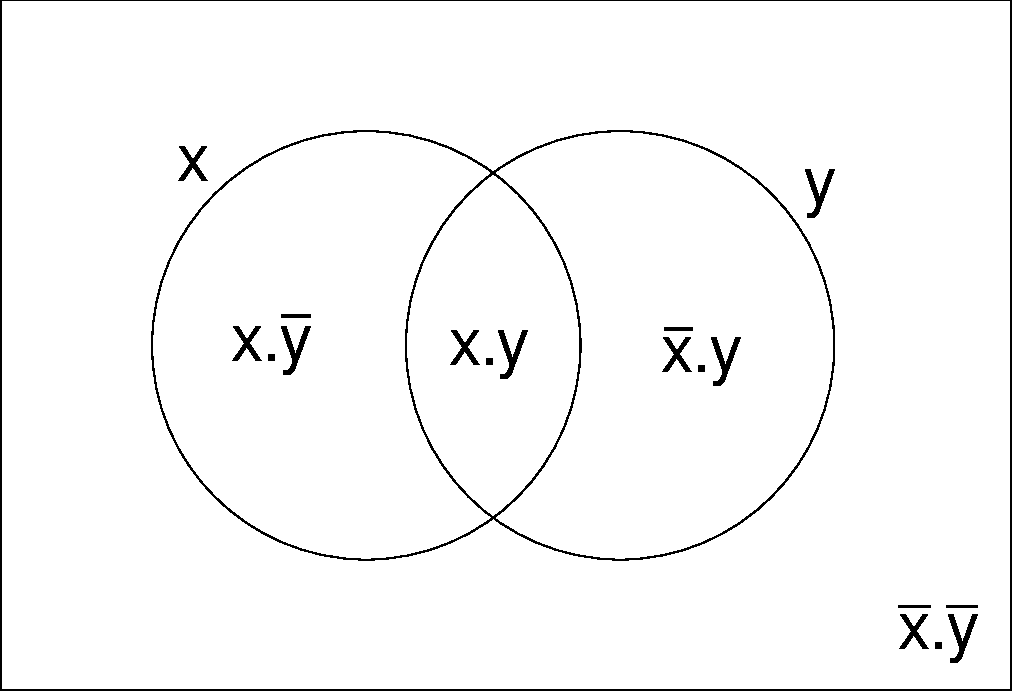
\includegraphics[width=.7\linewidth]{images/relacoesGerais}
			\caption{Relações de um espaço com duas variáveis}
			\label{fig:relacoesgerais}
		\end{figure}
		\column{.5\linewidth}
		\par A partir disso é possível escrever outras relações:
		\begin{equation}
			\begin{aligned}
				(x.\overline{y})+(x.y)&=x \\
				(\overline{x}.y)+(x.y)&=y \\
				(x.\overline{y})+(x.y)+(\overline{x}.y)&=x+y
			\end{aligned}
		\end{equation}
		
	\end{columns}
	
\end{frame}

\begin{frame}
	\frametitle{Provas de expressões na álgebra de Boole com diagrama de Venn }
	\par Como exemplo provaremos o do teorema de DeMorgan: $\overline{(x . y)} = \overline{x}+\overline{y}$
	\begin{columns}
		\column{.5\linewidth}
		\par Lado esquerdo da igualdade.	
		\begin{figure}
			\centering
			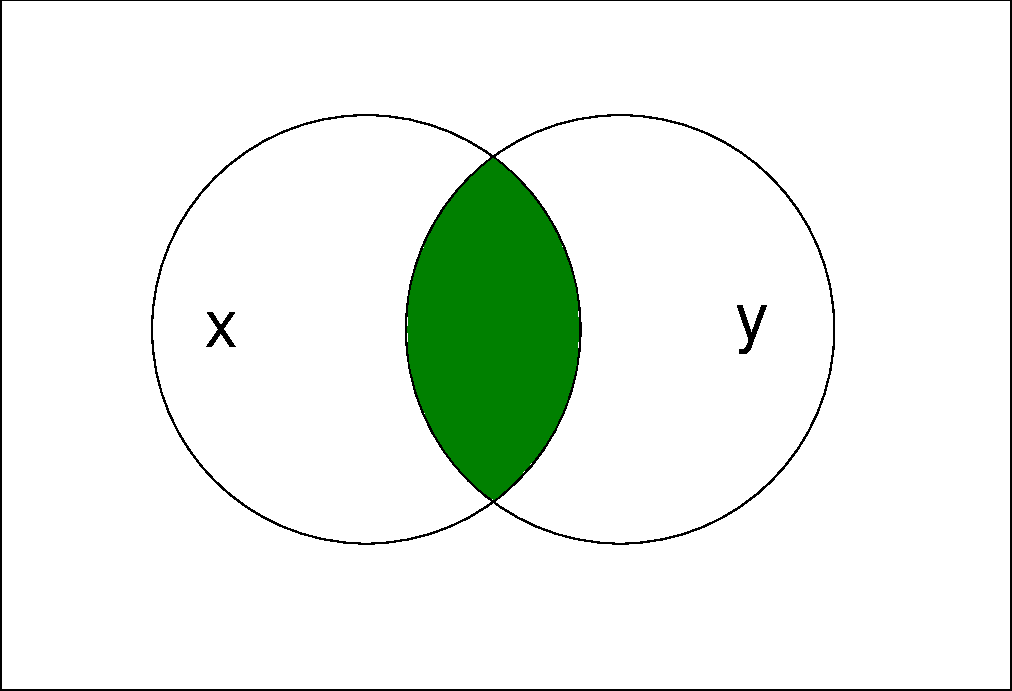
\includegraphics[width=0.4\linewidth]{images/x.y}
			\caption{$(x . y)$}
			\label{fig:x}
		\end{figure}
		\begin{figure}
			\centering
			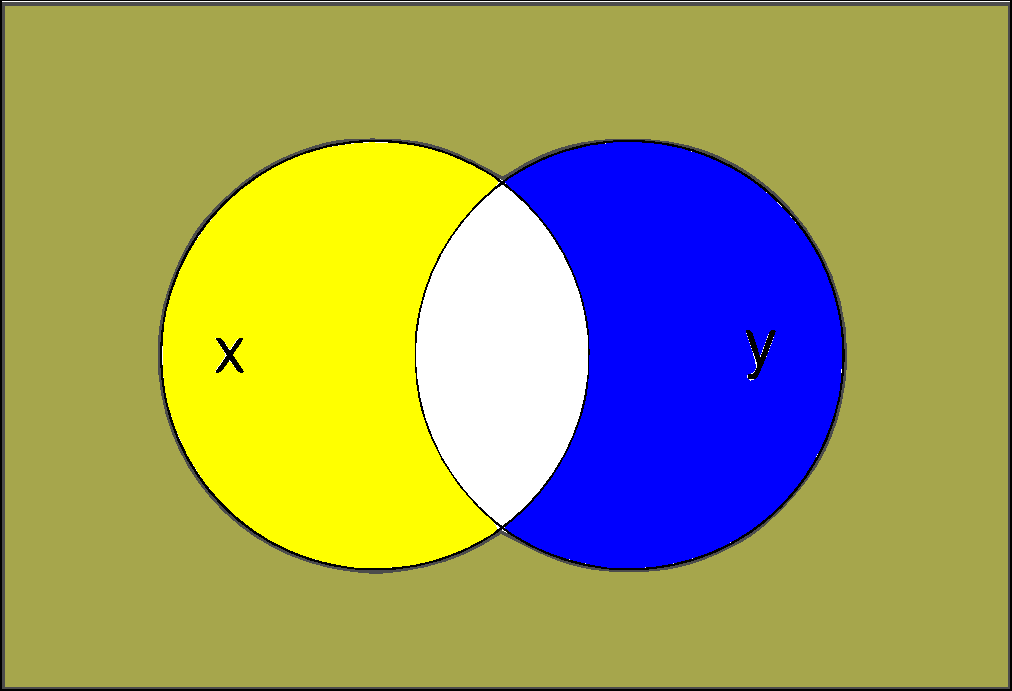
\includegraphics[width=0.4\linewidth]{images/notX.Y}
			\caption{$\overline{(x . y)}$}
			\label{fig:notx}
		\end{figure}
		\column{.5\linewidth}
		\par Lado direito da igualdade.
		\begin{figure}
			\centering
			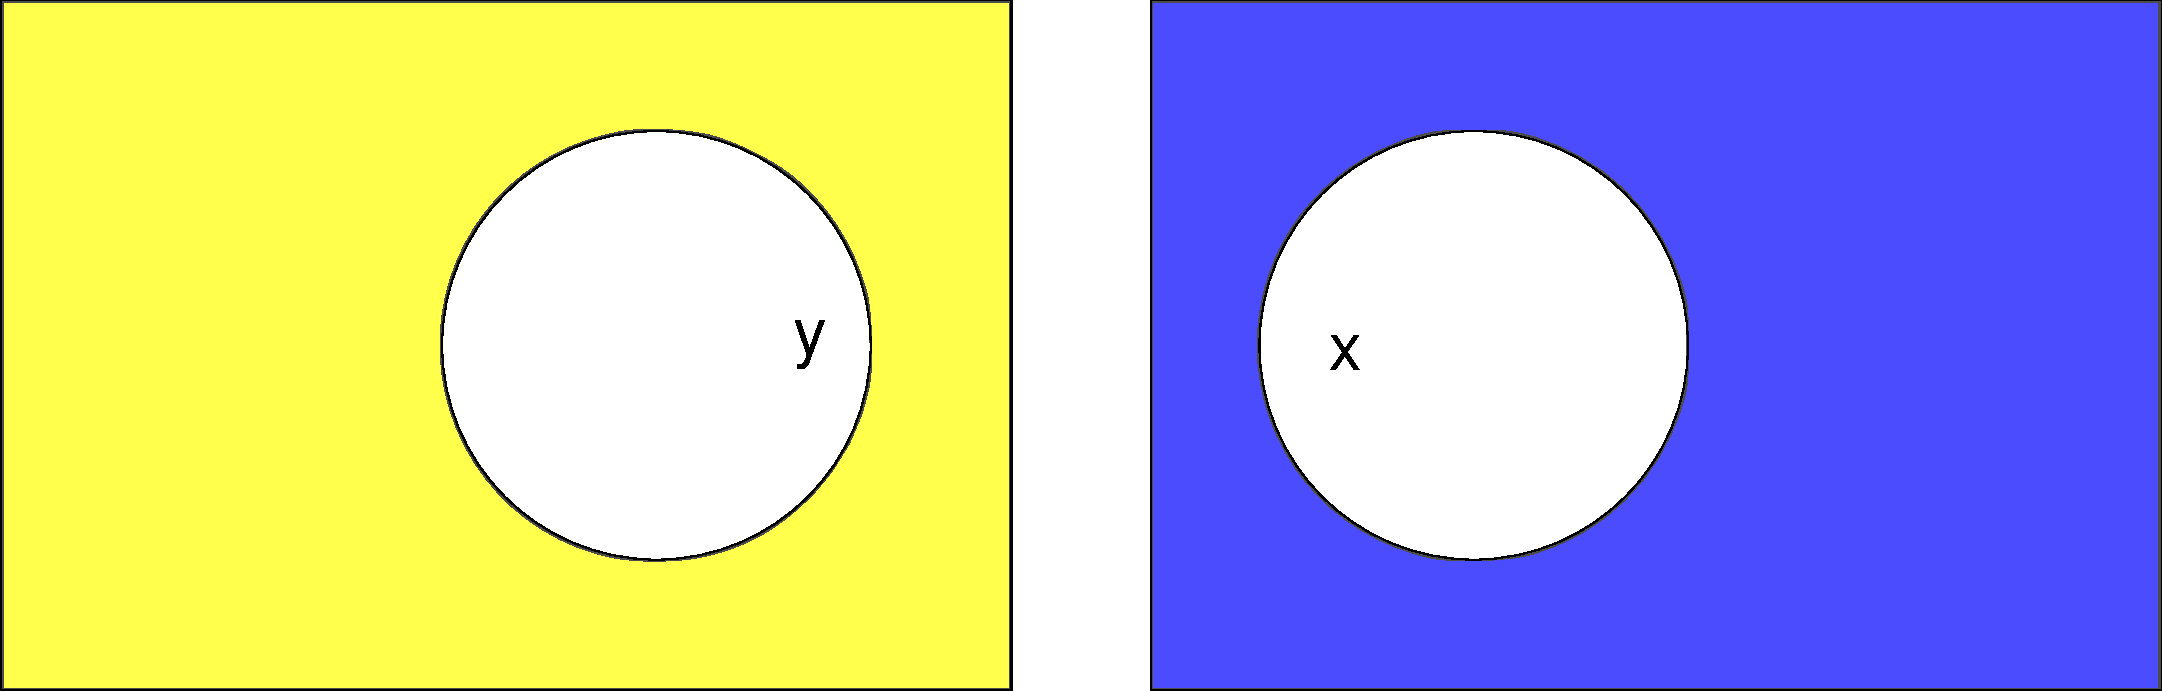
\includegraphics[width=.9\linewidth]{images/notXNotY}
			\caption{$\overline{x}$ e $\overline{y}$}
			\label{fig:notxnoty}
		\end{figure}
		\begin{figure}
			\centering
			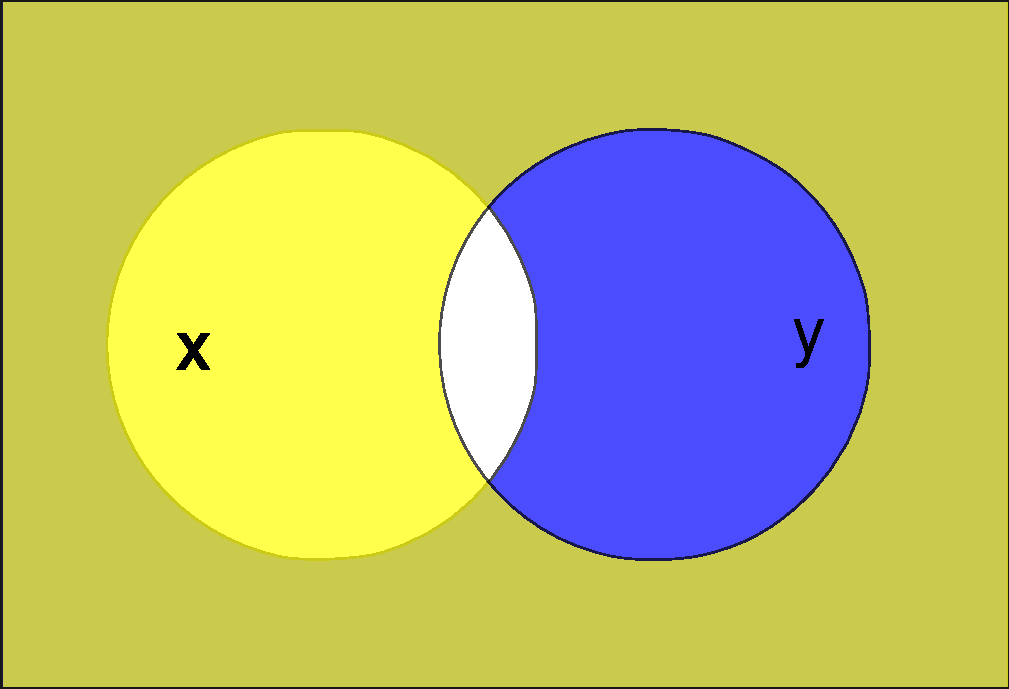
\includegraphics[width=0.4\linewidth]{images/notX+notY-4}
			\caption{$\overline{x}+\overline{y}$}
			\label{fig:notxnoty-4}
		\end{figure}
	\end{columns}
\end{frame}

\begin{frame}
	\frametitle{Provas de expressões na álgebra de Boole com diagrama de Venn }
	\par Como exemplo provaremos $(x.y)+(y.z)+(\overline{x}.z)=(x.y)+(\overline{x}.z) &\Leftrightarrow (x+y).(y+z).(\overline{x}+z) = (x+y).(\overline{x}+z) \text{ consenso (sumiço :D)}$
	\begin{columns}
		\column{.5\linewidth}
		\par Lado esquerdo da igualdade.
		\begin{figure}
			\centering
			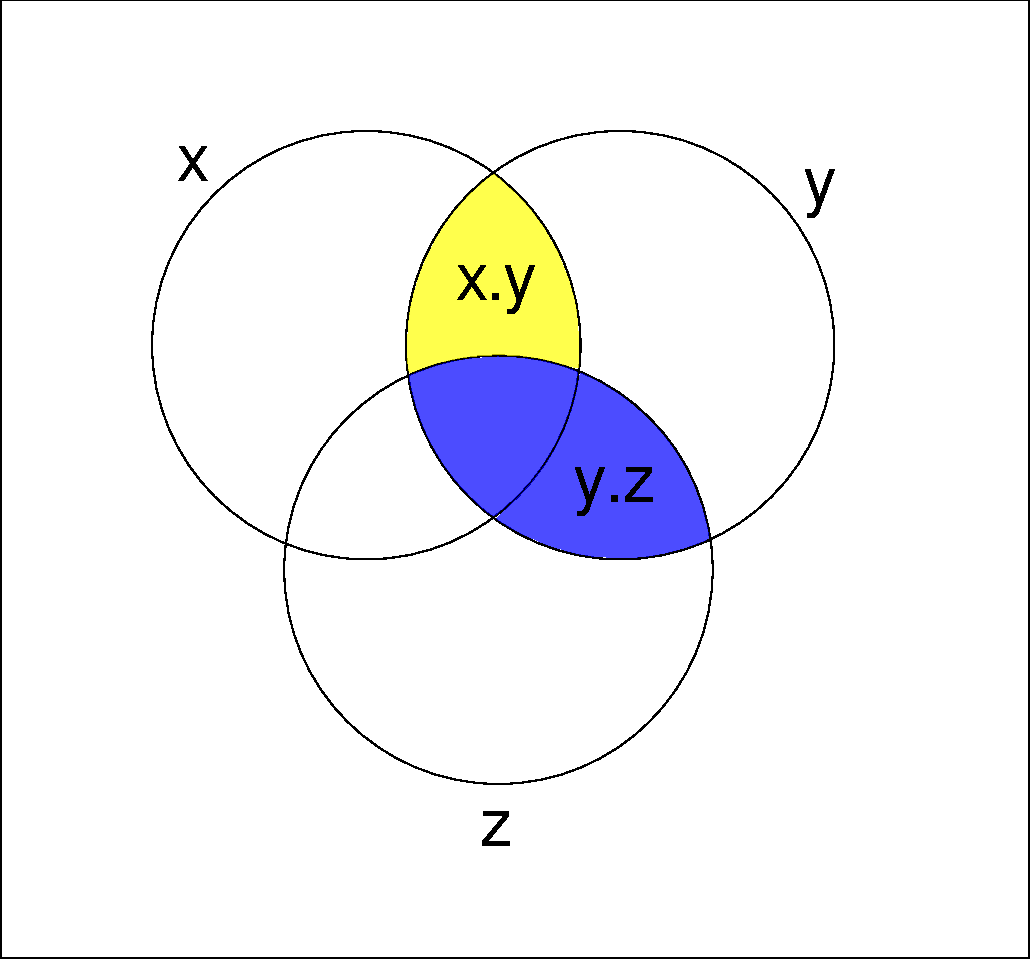
\includegraphics[width=0.35\linewidth]{images/x.y+y.z}
			\caption{$(x.y)+(y.z)$}
			\label{fig:xy+yz}
		\end{figure}
		
		\vspace{-2.3em} % Ajusta o espaçamento aqui
		
		\begin{figure}
			\centering
			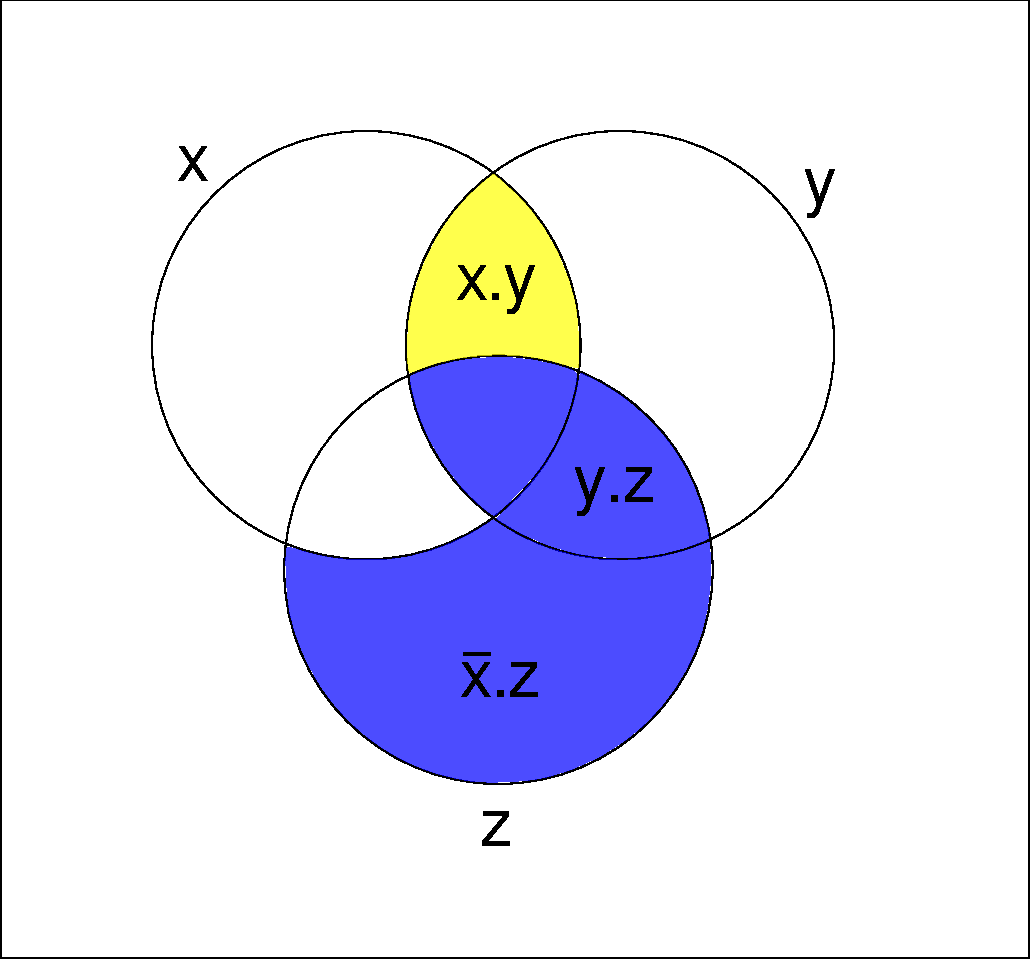
\includegraphics[width=0.35\linewidth]{images/x.y+y.z+notx.z}
			\caption{$(x.y)+(y.z)+(\overline{x}.z)$}
			\label{fig:x.y+y.z+notx.z}
		\end{figure}
		\column{.5\linewidth}
		\par Lado direito da igualdade.
		\begin{figure}
			\centering
			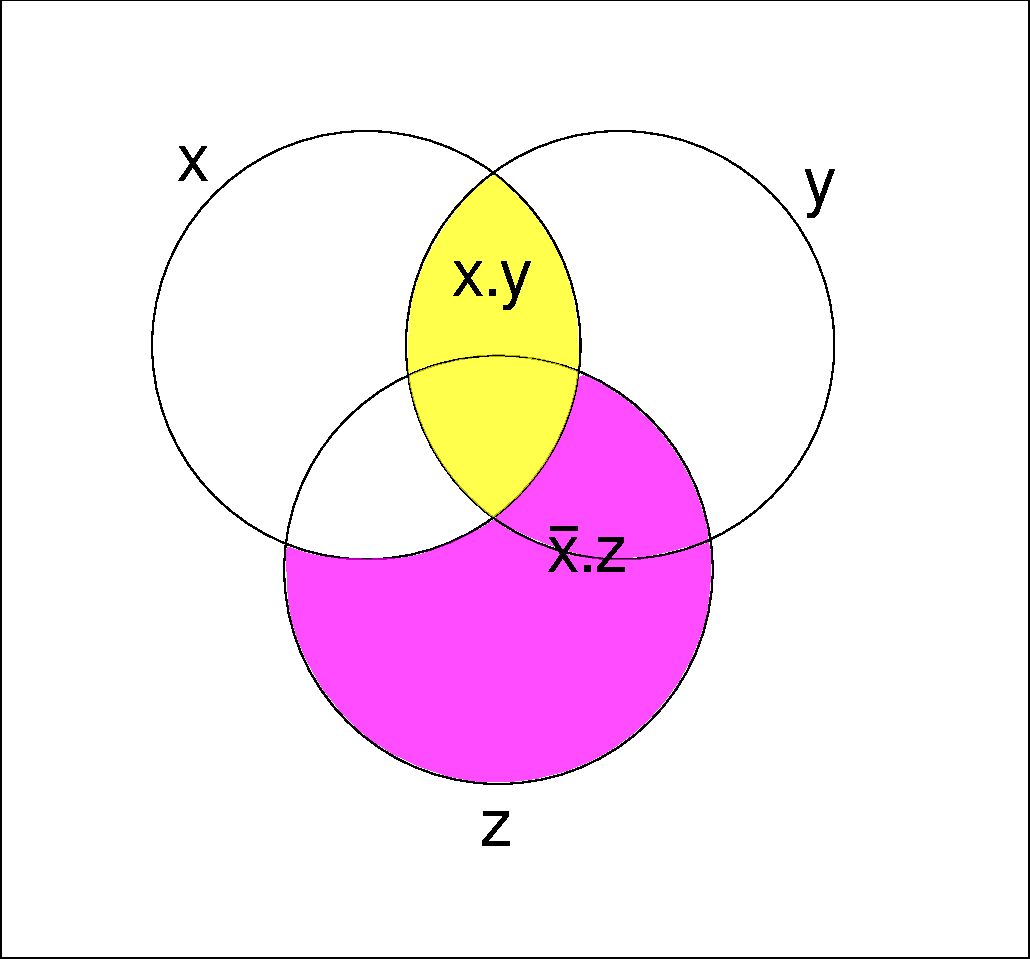
\includegraphics[width=0.5\linewidth]{images/x.y+notx.z}
			\caption{$(x.y)+(\overline{x}.z)$}
			\label{fig:x.y+notx.z}
		\end{figure}
		
	\end{columns}
\end{frame}

\begin{frame}
	\frametitle{Short test}
	\par A partir dos teoremas e propriedades apresentados mostre que $(x+y).(x+z)=x+y.z$. Indique quais os teoremas e/ou propriedades usados na solução.\newline
	\par Crie dualidades para
	\begin{itemize}
		\item $0.0$
		\item $1.1$
		\item $x=0 \implies \overline{x}=0$
	\end{itemize}
\end{frame}

\begin{frame}
	\frametitle{Circuitos}
	\par Até agora, revisamos a lógica, as tabelas-verdade e a álgebra booleana. No entanto, ainda não abordamos os circuitos digitais propriamente ditos. A partir de agora, exploraremos a correlação entre as expressões lógicas da álgebra booleana e o projeto de circuitos elétricos.
\end{frame}

\begin{frame}
	\frametitle{Circuitos combinacionais}
	\begin{columns}
		\column{0.6\textwidth}
		\par A chave binária é um componente que permite ou impede a passagem da corrente elétrica dado seus estado. A partir dela criaremos circuitos mais complexos.
		\begin{figure}
			\centering
			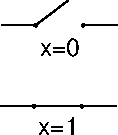
\includegraphics[width=0.2\linewidth]{images/chaveBinaria}
			\caption{Chave binária}
			\label{fig:chavebinaria}
		\end{figure}
		\column{0.4\textwidth}
		\par A chave binária pode ser representada de outra forma:
		\begin{figure}
			\centering
			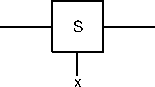
\includegraphics[width=0.7\linewidth]{images/chaveBinariaAbstrata}
			\caption{Chave binária}
			\label{fig:chavebinariaabstrata}
		\end{figure}
	\end{columns}
\end{frame}

\begin{frame}
	\frametitle{Circuitos combinacionais}
	\begin{columns}
		\column{0.6\textwidth}
		\par Agora considere uma função que depende um argumento $x$ para definir seu estado. Tal função pode ser representada no circuito abaixo:
		
		\begin{figure}
			\centering
			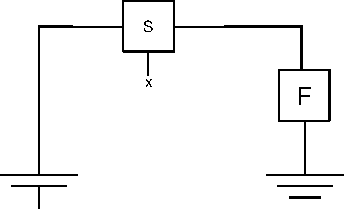
\includegraphics[width=0.7\linewidth]{images/funcaoLogica1var}
			\caption{Função lógica de uma variável. No circuito $F$ pode ser ligada a qualquer elemento de saída com um led ou outro circuito.}
			\label{fig:funcaologica1var}
		\end{figure}
		
		\column{0.4\textwidth}
		\par $F = 1 \forall x=1$
		\par $F = 0 \forall x=0$
		\par Portanto $F$ é uma função lógica de \textbf{uma} variável tal que $F(x)=x$
		
	\end{columns}
\end{frame}

\begin{frame}
	\frametitle{Circuitos combinacionais}
	\par A partir de agora é possível construir circuitos mais complexos como \textbf{OR} e \textbf{AND}.
	\begin{columns}
		\column{0.5\textwidth}
		\begin{figure}
			\centering
			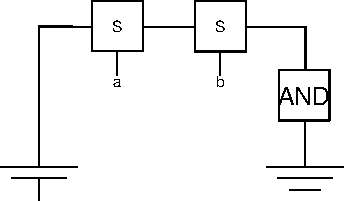
\includegraphics[width=0.7\linewidth]{images/portaE}
			\caption{Circuito \textbf{AND}: $a$ e $b$ são suas entradas. Aqui se pode constatar que este circuito pode receber de $2$ a $n$ entradas.}
			\label{fig:portae}
		\end{figure}
		\column{0.5\textwidth}
		\begin{figure}
			\centering
			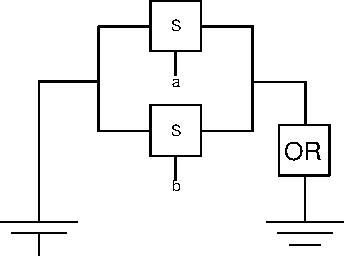
\includegraphics[width=0.7\linewidth]{images/portaOU}
			\caption{Circuito \textbf{OR}: $a$ e $b$ são suas entradas. Aqui se pode constatar que este circuito pode receber de $2$ a $n$ entradas.}
			\label{fig:portaou}
		\end{figure}
	\end{columns}
\end{frame}

\begin{frame}
	\frametitle{Circuitos combinacionais}
	\par Circuito \textbf{NOT}
	\begin{columns}
		\column{0.5\textwidth}
		\begin{figure}
			\centering
			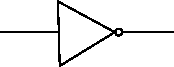
\includegraphics[width=0.7\linewidth]{images/portaNao}
			\caption{Circuito \textbf{NOT}: Inverte a entrada $a$.}
			\label{fig:portanao}
		\end{figure}
		
		\column{0.5\textwidth}
		\par Nada aqui por questões estéticas...
	\end{columns}
\end{frame}

\begin{frame}
	\frametitle{Circuitos combinacionais}
	\par E assim como vimos na álgebra de Boole \textbf{OR} e \textbf{AND} podem ser combinados.
	\begin{figure}
		\centering
		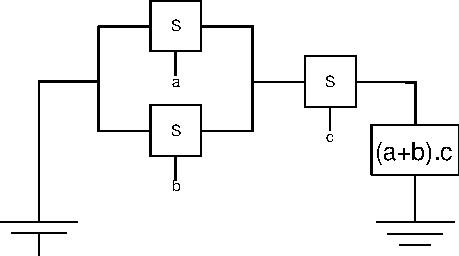
\includegraphics[width=0.7\linewidth]{images/aMaisBVezesC}
		\caption{O \textbf{OR} recebe as entradas $a$ e $b$, o circuito \textbf{AND} recebe $c$ e a saída de \textbf{OR}}
		\label{fig:amaisbvezesc}
	\end{figure}
\end{frame}

\begin{frame}
	\frametitle{Circuitos combinacionais}
	\par Para representar circuitos simples os símbolos já vistos são suficientes, porém, quando a complexidade aumenta pode ficar beeeeeemmmm complicado entender o que se passa. Então precisamos aumentar o nível de abstração encapsulando esse componentes.
\end{frame}

\begin{frame}
	\frametitle{Circuitos combinacionais}
	\begin{figure}
		\centering
		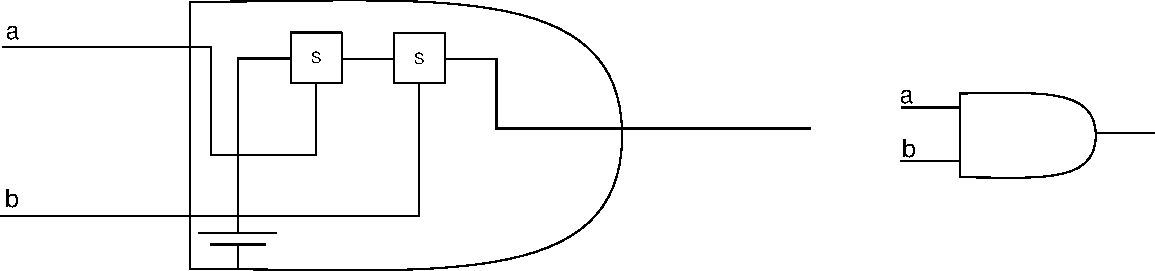
\includegraphics[width=0.7\linewidth]{images/portaEAbstrata}
		\caption{Abstração de circuito \textbf{AND} para a porta \textbf{AND}}
		\label{fig:portaeabstrata}
	\end{figure}
\end{frame}

\begin{frame}
	\frametitle{Circuitos combinacionais}
	\begin{figure}
		\centering
		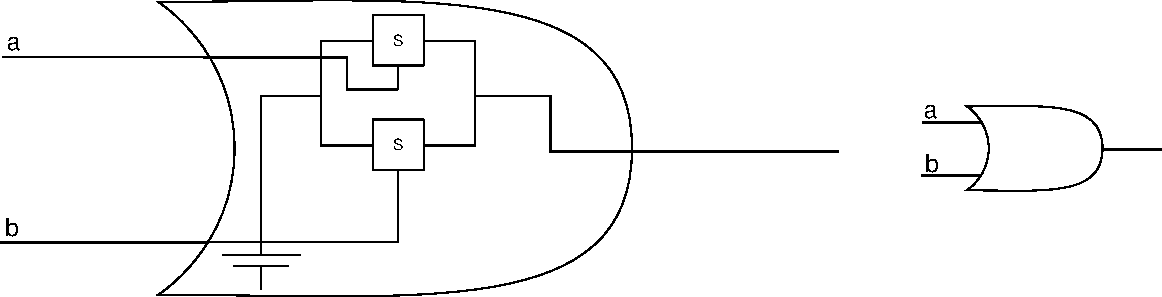
\includegraphics[width=0.7\linewidth]{images/portaOUAbstrata}
		\caption{Abstração de circuito \textbf{OR} para a porta \textbf{OR}}
		\label{fig:portaouabstrata}
	\end{figure}
\end{frame}

\begin{frame}
	\frametitle{Circuitos combinacionais}
	\begin{figure}
		\centering
		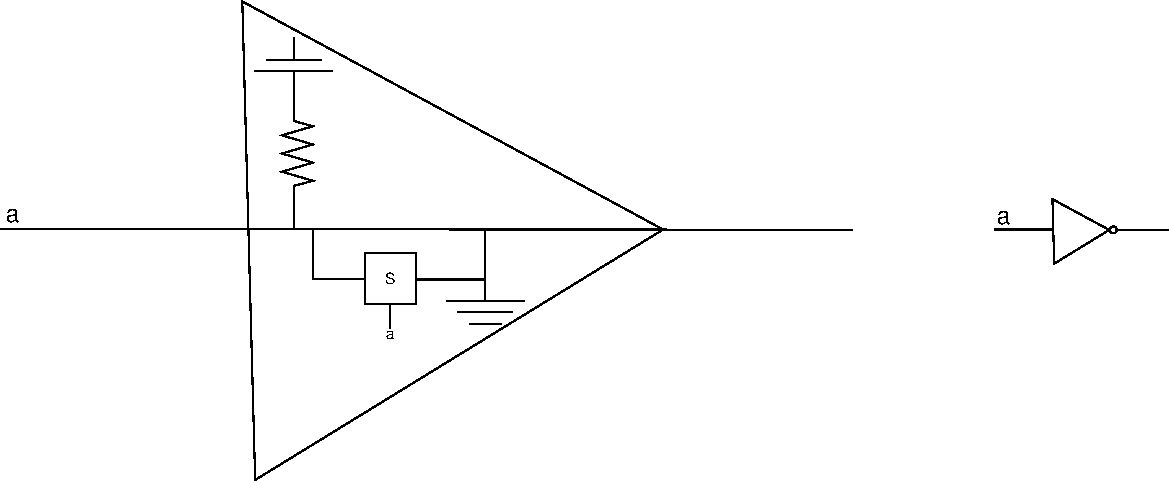
\includegraphics[width=0.7\linewidth]{images/portaNOTAbstrata}
		\caption{Abstração de circuito \textbf{NOT} para a porta \textbf{NOT}}
		\label{fig:portanotabstrata}
	\end{figure}
\end{frame}

\begin{frame}
	\frametitle{Circuitos combinacionais}
	\par Veja como fica o circuito $(a+b).c$ com as novas abstrações.
	\begin{figure}
		\centering
		% Define cores personalizadas
\definecolor{vermelho}{HTML}{FF0000}
\definecolor{verde}{HTML}{00FF00}


\begin{tikzpicture}[circuit logic US, scale=1]
	% Define nós de entrada
	\node (a) at (0,0) {$a$};
	\node (b) [below=0.5cm of a] {$b$};
	\node (c) [below=0.5cm of b] {$c$};
	
	% Define portas lógicas usando coordenadas relativas
	\node (or) [or gate, right=1cm of a.east, yshift=-0.5cm, draw=vermelho, fill=vermelho!20] {};
	\node (and) [and gate, right=1cm of or.output, yshift=-.5cm, draw=verde, fill=verde!20] {};
	
	% Desenhar as conexões
	\draw [draw=black, line width=.3mm] (a.east) -- ++(0.5,0) |- (or.input 1);
	\draw [draw=black, line width=.3mm] (b.east) -- ++(0.5,0) |- (or.input 2);
	
	\draw [draw=black, line width=.3mm] (or.output) -- ++(0.5,0) |- (and.input 1);
	\draw [draw=black, line width=.3mm] (c.east) -- ++(0.5,0) |- (and.input 2);
	\draw [draw=black, line width=.3mm] (and.output) -- ++(0.5,0) node[right] {$\text{saída}$};
\end{tikzpicture}
		\caption{Circuito correspondente a expressão lógica (a+b).c}
		\label{fig:circuitoAndOr}
	\end{figure}
\end{frame}
